% 第 22 题四棱锥图：按固定源 400 dpi 位图实测值复刻（1 bp → 0.03515 cm）。
% 原点取顶点 A（源页 (1016.2, 274.1)），y 向上。
% 源为精确斜二测（深度轴 135°、压缩 0.501，单位长 58.4 pt；AD/BC=2、PA/BC=2 均严格）；
% 实线 6 段（三条可见侧棱 + 底棱 BC/CD + 题面(2)的 QC）；虚线 3 段（被遮挡的 PA、AB、AD，共端点 A）；虚线样式照源 [2.99 2.99]（三方向节距一致）。
% 图内无实心点、无直角记号（题面文本保证直角）；Q 恰为 PB 中点（作图取位，照源）。
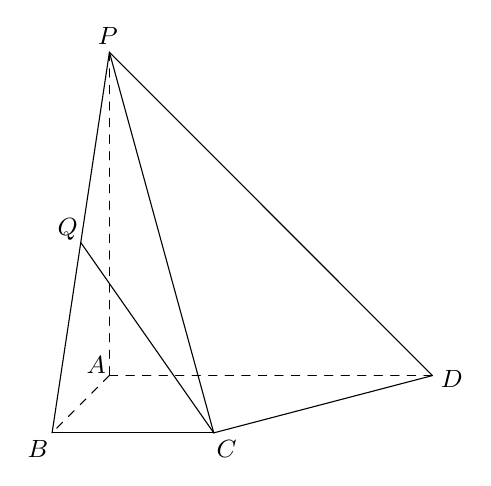
\begin{tikzpicture}[line cap=round,line join=round,font=\small,x=0.03515cm,y=0.03515cm]
% ===== 实线（6 段）=====
\draw (0,116.8)--(-20.7,-20.7);   % P–B 侧棱
\draw (0,116.8)--(37.7,-20.7);   % P–C 侧棱
\draw (0,116.8)--(116.7,0);   % P–D 侧棱
\draw (-20.7,-20.7)--(37.7,-20.7);   % B–C 底棱（水平）
\draw (37.7,-20.7)--(116.7,0);   % C–D 底棱
\draw (-10.3,48)--(37.7,-20.7);   % Q–C 题面(2) 直线 CQ
% ===== 虚线（3 段，共端点 A）=====
\draw[dash pattern=on 2.99pt off 2.99pt] (0,116.8)--(0,0);   % P–A 被遮挡侧棱（竖直）
\draw[dash pattern=on 2.99pt off 2.99pt] (0,0)--(-20.7,-20.7);   % A–B 被遮挡底棱（135°）
\draw[dash pattern=on 2.99pt off 2.99pt] (0,0)--(116.7,0);   % A–D 被遮挡底棱（水平）
% ===== 标注（照源字框中心，显式坐标）=====
\node[anchor=center,inner sep=0] at (-0.6,122.6) {\(P\)};
\node[anchor=center,inner sep=0] at (-15.1,52.9) {\(Q\)};
\node[anchor=center,inner sep=0] at (-4.8,3.8) {\(A\)};
\node[anchor=center,inner sep=0] at (-25.8,-26.7) {\(B\)};
\node[anchor=center,inner sep=0] at (42.4,-26.7) {\(C\)};
\node[anchor=center,inner sep=0] at (123.7,-1.1) {\(D\)};
\end{tikzpicture}
